%----------------------------------------------------------------------
\section{$DLEQ$ non-interactive proof between voters and verifier}
\label{sec:dleq_non-interactive-proof-between_voters_and_verifier}
%----------------------------------------------------------------------
In section \ref{sec:dleq_voter_verifier} we elaborated an interactive $DLEQ$ proof between voter and verifer. Here we present how one can turn an interactive proof to a non interactive proof. This is also known as the Fiat Shamir where we are transforming an interactive proof into a non interactive proof which is described in section ~\ref{sec:fiat_shamir}. Instead of the verifier computes a challenge, the prover computes the challenge as a random function as described in \ref{sec:hash_function}.  We will present two ways off doing this transformation, a non optimized and an optimized version. Last we will describe an example on how this can be done.\\


\parahead{The prover computes} \begin{math}a_1=g^w \ (mod\ q)  \ and \ a_2=y_i^w \ (mod\ q),  w\in_R \Z_q \end{math}. Then the prover computes the hash \begin{math}C=H(X_i,Y_i,a_1,a_2) \end{math}. Then the prover computes  \begin{math}r=w-p(i)  \cdot  C \ (mod\ q)\end{math}. Last the prover publish \begin{math}a_1, a_2,r,C\end{math}. \\

\noindent
\parahead{The verifier computes} the following computations \begin{math}a_1 = g^r \cdot X_i^C  \ (mod\ q)\end{math} and \begin{math} a_2=y_i^r  \cdot  Y_i^C \ (mod\ q)\end{math} and \begin{math}C=H(X_i,Y_i,a_1,a_2)\end{math}.


\begin{figure}[H]
    \centering        
    
    $
    \begin{array}{l}
    \hline                      \
    \textbf{DLEQ protocol}      \\
    \hline                      \
    Input:  g,X_i,y_i,Y_i   \ where \ X_i = g^{x_i} \ and \ Y_i=y_i^{x_i}
    \\
	\begin{array}{L{1.1cm}lcl}
        & \text{\textsf{Prover}} & & \text{\textsf{Verifier}} \\
        \hline
        Step \ 1    &           \begin{array}{l}
                                    w\in_R \Z_q             \\ 
                                    a_1=g^w \ (mod\ q)      \\ 
                                    a_2=y_i^w \ (mod\ q)    \\
                                    C=H(X_i,Y_i,a_1,a_2)    \\
                                    r=w-p(i)  \cdot  C \ (mod\ q)
                                \end{array}     &               & \\
                    &                   &               & \\
        Step \ 2    &                   &               \xrightarrow{\hspace{0.4em}a_1 , a_2 , r , C\hspace{0.4em}} & \begin{array}{l}
            checks \ if: \\      
            a_1 = g^r \cdot X_i^C \\ 
            a_2=y_i^r \cdot Y_i^C \\
            C=H(X_i,Y_i,a_1,a_2)
        \end{array} \\
        \hline
    \end{array}
    \end{array}
    $    
    \caption{$DLEQ$ non interactive}
	\label{fig:DLEQ_1}
\end{figure}


\noindent
Note in above that there is no interaction between the prover and the verifier. \\

\noindent 
\textbf{$DLEQ$ optimized}\\
In the following we will show how one can improve the amount of computation of the challenge \textit{C}. Instead of computing the challenge \textit{n} times, one can compute it once and reuse the challenge.

\begin{enumerate}
    \item The prover publish  \begin{math}a_{1,i}=g^{w_i} \ (mod\ q)  \ and \ a_{2,i}=y_i^{w_i} \ (mod\ q)\end{math}  for  \begin{math} 1\leq i \leq n, \ w_i\in_R \Z_q \end{math}.
    \item The prover computes the hash \begin{math}C=H(X_i,Y_i,...,X_n,Y_n,a_{1,1},a_{2,1},\\a_{1,2},a_{2,2},...,a_{1,n},a_{2,n})\end{math}.
    \item The prover computes \begin{math}r_i\end{math}:  \begin{math}r_i=w_i-p(i)  \cdot  C \ (mod\ q)\end{math} and publish \begin{math}r_i,C\end{math}.
    \item The verification contains of the following computation:
    \begin{enumerate}        
        \item The verifier checks if:   \begin{math}a_{1,i} = g^{r,i} \cdot X_i^C \ (mod\ q) \end{math}
        \item The verifier checks if:  \begin{math} a_{2,i}=y_i^{r_{i}}  \cdot  Y_i^C \ (mod\ q)\end{math}
         \item The verifier checks if:  $C=H(X_i,Y_i,...,X_n,Y_n,a_{1,1},a_{2,1},$\\
$a_{1,2},a_{2,2},...,a_{1,n},a_{2,n})$
    \end{enumerate}
\end{enumerate}

\noindent 
\textbf{$DLEQ$ computation voter}\\
Hence the hash contains all the  \begin{math}a_i \end{math} the prover will compute this proof once for all  \begin{math}p(i) \end{math} which improve efficiency. This means that if there are $3$ shares, then the above computation has to be done $3$ times, one for each tally, but same hash can be computed once for every tally. 



\begin{enumerate}
    \item The prover publish $a_{1,1},a_{2,1},a_{1,2},a_{2,2},a_{1,3},a_{2,3}$.
    \item The prover publish $C,r_1,r_2,r_3$.
    \item The prover selects  $w_1, w_2,w_3\in_R \Z_q$.
    \item The prover computes $a_{1,i}=g^w_i \ (mod\ q) \ and \ a_{2,i}=y_i^{w_i} \ (mod\ q)$.
    \item The prover computes the hash  $C=H(X_i,Y_i,...,X_n,Y_n,a_{1,1},a_{2,1},$\\
$a_{1,2},a_{2,2},...,a_{1,n},a_{2,n})$.
    \item The prover computes $\ r_i:  r_i=w_i-p(i)  \cdot  C \ (mod\ q)$ .
    \item The verification contains of the following computation:
    \begin{enumerate}        
        \item The verifier checks if: $a_{1,i} = g^{r,i} \cdot X_i^C \ (mod\ q) $
        \item The verifier checks if: $a_{2,i} =y_i^{r_{i}}  \cdot  Y_i^C \ (mod\ q)  $ 
         \item The verifier checks if: $C=H(X_i,Y_i,...,X_n,Y_n,a_{1,1},a_{2,1},$\\
$a_{1,2},a_{2,2},...,a_{1,n},a_{2,n})$
    \end{enumerate}
\end{enumerate}



\noindent
\textbf{Zero knowledge proof for the $DLEQ$}\\
The same arguments holds for correctness, soundness and zero knowledge, which is described in section \ref{sec:dleq_voter_verifier} about the interactive $DLEQ$. 



%----------------------------------------------------------------------
\section{$DLEQ$ proof by the talliers}
\label{sec:dleq_proof_by_the_talliers}
%----------------------------------------------------------------------
The talliers will do computations on each of their shares. Each tally uses the $DLEQ$ to prove that the decryption of their shares is done correctly. It proofs that the exponent are equal \begin{math}G = y_i^{x_i}  \ and \ Y_i=S_i^{x_i} \end{math} without revealing \begin{math}x_i \end{math} and if the prover was honest, then it should be the case that we get same computed values in the end meaning \begin{math}a_1=G^w = G^r \cdot y_i^C\end{math} and \begin{math}a_2=S_i^w = S_i^r \cdot Y_i^C\end{math}.\\

\noindent
First we show the interactive proof and then transform it to a non-interactive proof. The input values are \begin{math}(G,\ y_i,\ S_i, Y_i)\end{math} where \begin{math}G = y_i^{x_i}\end{math} and  \begin{math} Y_i=S_i^{x_i}\end{math}. We have some initial values
 \begin{math}g_1 =G,\ h_i=y_i,\ g_2=S_i,\ h_2=Y_i,\ \alpha=x_i \end{math} and \begin{math}w \in_R \{0,...,q-1\}\end{math}.\\
 
 
 
\noindent 
In step 1 the prover computes \begin{math}a_1=G^w,\ a_2=S_i^w\end{math}. In step 2
the verifier creates a challenge \begin{math}C\end{math}. In step 3 the tally computes \begin{math}r=w-C \cdot x_i\end{math}. In step 4 the verifier computes \begin{math}a_1=G^r \cdot y_i^C,\ a_2=S_i^r \cdot Y_i^C\end{math}.
 
 
 
\begin{figure}[H]
    \centering        
    
    $
    \begin{array}{l}
    \hline                      \
    \textbf{DLEQ protocol by the talliers}      \\
    \hline                      \
    Input:  G,\ y_i,\ S_i, \ Y_i \ where \ G = y_i^{x_i} \ and \ Y_i=S_i^{x_i}     \\
    Output: 0 \ or \ 1
    \\
	\begin{array}{L{2cm}ccc}
        & \text{\textsf{Prover}} & & \text{\textsf{Verifier}} \\
        \hline
        Step \ 1 & w\in_R \Z_q & & \\
        & a_1=G^w     & & \\
        & a_2=S_i^w   & \xrightarrow{\hspace{1em}a_1 , a_2\hspace{1em}} & \\
        Step \ 2 & & & C\in_R \Z_q \\
        & & \xleftarrow{\hspace{2em}C\hspace{2em}} & \\
        Step \ 3 & r=w-x_i  \cdot  C    & & \\
        Step \ 4 & & \xrightarrow{\hspace{2em}r\hspace{2em}} & \begin{array}{c}
        checks \ if: \\      
        a_1 = G^r \cdot y_i^C \\ 
        a_2=S_i^r \cdot Y_i^C
        \end{array} \\
        \hline
    \end{array}
    \end{array}
    $    
    \caption{$DLEQ$}
	\label{fig:DLEQ_by_talliers}
\end{figure} 

\noindent
Note the interaction in step 2 where the verifier creates a challenge to the prover. Through Fiat–Shamir we transform an interactive proof of knowledge into a non-interactive proof of knowledge by replacing step 2 with a hash algorithm  \begin{math}C=H(G,\ y_i,\ S_i,\ Y_i,\ a_1,\ a_2)\end{math}.\\
 
 \noindent
\textbf{Mathematical justification}\\
To justify correctness of the computations in step 4, we can do the following verification on \begin{math}a_1=G^w \stackrel{?}{=} G^r \cdot y_i^C\end{math} and \begin{math}a_2=S_i^w \stackrel{?}{=} S_i^r \cdot Y_i^C\end{math}.


\begin{alignat*}{5}
a_1 &=G^r \cdot y_i^C &=G^r \cdot y_{x_i}^C &=G^{r+x_iC} =G^{w-Cx_i+x_iC} =G^w\\
a_2 &= S_i^r \cdot Y_i^C &=S^r \cdot Y_{x_i^C} &=S^{w-Cx_i} \cdot S_i^{x_i \cdot C} =S^{w-Cx_i+x_i \cdot C}&=S_i^w
\end{alignat*}



\noindent
To show soundness and zero knowledge the same process from section \ref{sec:dleq_voter_verifier} can be followed.


\chapter{Calculations}
%----------------------------------------------------------------------
\section{Simple review of calculations in the protocol}
\label{sec:simple_review_of_calculations_in_the_protocol}
%----------------------------------------------------------------------
We will present a simplified example of the calculations through the protocol, which illustrate casting the votes and tallying the final counts of the votes. The structure follows the protocol as described in section \ref{sec:the_protocol}. This example does not contain calculations of the proof. These are described in section \ref{sec:proofs}. In this calculation there are $3$ voters ($m$) and $3$ talliers ($n$). The example shows  3 voters which cast their votes and how 3 talliers are able to reconstruct the sum of all votes.\\

\noindent
\textbf{The bulletin board publishes all system parameters which is the public elements a prime $q$,  the generators $g$ and $G$ and a security parameter $t$.}


\begin{table}[H]
\centering
\begin{tabular}{|l|l|}
\hline
\multicolumn{2}{|l|}{\textbf{Public elements}} \\ \hline
Prime $q$                       & $5$              \\ \hline
Security parameter $t$          & $3$              \\ \hline
Generator $G$                   & $5$              \\ \hline
Generator $g$                   & $9$              \\ \hline
Lambda  $\lambda_1, \ \lambda_2,\ \lambda_3$                      & $3,-3,1$         \\ \hline
\end{tabular}
\caption{The lambda is based on the calculation from section \ref{sec:shamir_secret_sharing_lagrange_interpolation} }
\label{my-label}
\end{table}

\noindent
\textbf{The tallier generates a private key $x_i$ and a public key $y_i$.}

\begin{table}[H]
\centering
\begin{tabular}{|l|l|l|}
\hline
\multicolumn{3}{|l|}{\textbf{Talliers}}        \\ \hline
\textbf{} & Public key $y_i$ & Private key $x_i$ \\ \hline
Tally 1 & 5               & 1                \\ \hline
Tally 2 & 3               & 2                \\ \hline
Tally 3 & 4               & 3                \\ \hline
\end{tabular}
\caption{Public and private keys for the talliers}
\label{my-label}
\end{table}

\noindent
\textbf{The voters casts their votes, either 0 or 1. and creates a random secret $s$ and a random polynomial of degree at most $t-1$ and computes the shares.}

\begin{table}[H]
\centering
\begin{tabular}{|l|l|}
\hline
\multicolumn{2}{|l|}{\textbf{Voter 1}}        \\ \hline
Vote $v$          & $1$                         \\ \hline
Random secret $s$ & $2$                         \\ \hline
Random polynomial $p(x)$ & $2+2x+4x^2$ \\ \hline
\multicolumn{2}{|l|}{\textbf{Voter 2}}        \\ \hline
Vote $v$          & $1$                         \\ \hline
Random secret $s$ & $3$                         \\ \hline
Random polynomial $p(x)$ & $3+x+4x^2$ \\ \hline
\multicolumn{2}{|l|}{\textbf{Voter 3}}        \\ \hline
Vote $v$          & $1$                         \\ \hline
Random secret $s$ & $4$                         \\ \hline
Random polynomial $p(x)$ & $4+3x+4x^2$ \\ \hline
\end{tabular}
\caption{3 voters creates their vote, secret and polynomial}
\label{my-label}
\end{table}


\begin{table}[H]
\centering
\begin{tabular}{|l|l|l|l|l|}
\hline
\multicolumn{5}{|l|}{\textbf{The voters creates their shares $p(x)$}}                                    \\ \hline
\textbf{Voter/point}            & $p(0)$ & Tally $1$ & Tally $2$ & Tally $3$ \\ \hline
$p_1(x)= 2+2x+4x^2$ &  $2$    & $3$         & $2$         & $4$         \\ \hline
$p_2(x)= 3+x+4x^2$  &  $3$    & $3$         & $1$         & $2$         \\ \hline
$p_3(x)= 4+3x+4x^2$ &  $4$    & $1$         & $1$         & $4$         \\ \hline
\end{tabular}
\caption{The shares are computed $p_1(1)=3 \ (mod \ 5),\ p_1(2)=2 \ (mod \ 5),\ p_1(3)=4 \ (mod \ 5)$ etc.}
\label{my-label}
\end{table}

\noindent
\textbf{The voter distributes the encrypted share.}

\begin{table}[H]
\centering
\begin{tabular}{|l|l|l|l|}
\hline
\multicolumn{4}{|l|}{\textbf{\begin{tabular}[c]{@{}l@{}}Encryption of the shares $Y_i= y^{p(i)}$ using \\ the talliers public key\end{tabular}}} \\ \hline
\textbf{Voter/Talliers}          & Tally $1$                     & Tally $2$                     & Tally $3$                     \\ \hline
Voter $1$                         & $5^3=4$         & $3^2=9$         & $4^4=3$         \\ \hline
Voter $2$                         & $5^3=4$         & $3^1=3$         & $4^2=5$         \\ \hline
Voter $3$                         & $5^1=5$         & $3^1=3$         & $4^4=3$         \\ \hline
\end{tabular}
\caption{The encryption consist of raising the share in the exponent on the Talliers public key such as $y_i^{p_j(i)} \ (mod \ 11)$.}
\label{my-label}
\end{table}


\noindent
\textbf{The tallier multiplies the encrypted shares $Y_i^*$ and decrypt the multiplum of shares $S_i^*$.}\\

\begin{table}[H]
\centering
\begin{tabular}{|l|l|}
\hline
\multicolumn{2}{|l|}{\textbf{Tallier computes $Y^*$}}                        \\ \hline
Tally $1$ & $Y_1^* = (4 \cdot 4 \cdot 5) = 80 = 3 \ (mod \ 11)$                             \\ \hline
Tally $2$ & $Y_2^* = (9 \cdot 3 \cdot 3) = 81 = 4 \ (mod \ 11)$                             \\ \hline
Tally $3$ & $Y_3^* = (3 \cdot 5 \cdot 3) = 45 = 1 \ (mod \ 11)$                             \\ \hline
\multicolumn{2}{|l|}{\textbf{Tallier computes $S^*$}}                        \\ \hline
Tally $1$ & $(x_1)^{-1} = 1 \cdot x = 1 \ (mod \ 5) = 1, \ S_1^* = 3^1 = 3 \ (mod \ 11)$ \\ \hline
Tally $2$ & $(x_2)^{-1} = 2 \cdot x = 1 \ (mod \ 5) = 3, \ S_2^* = 4^3 = 9 \ (mod \ 11) $ \\ \hline
Tally $3$ & $(x_3)^{-1} = 3 \cdot x = 1 \ (mod \ 5) = 2, \ S_3^* = 1^2 = 1 \ (mod \ 11) $ \\ \hline
\end{tabular}
\caption{The talliers computes $Y^*$ and $S^*$.}
\label{my-label}
\end{table}

\noindent
\textbf{A master authority applies Lagrange interpolation}\\

\begin{table}[H]
\centering
\begin{tabular}{|l|l|}
\hline
\multicolumn{2}{|l|}{\textbf{Apply lambda to $S^*$}}                                                                     \\ \hline
$S_1^{* \cdot \lambda_1}$                                            & $3^{3 \ (mod \ 5)} = 3^3 \ (mod \ 11) = 5$  \\ \hline
$S_2^{* \cdot \lambda_2}$                                            & $9^{-3 \ (mod \ 5)} = 9^2 \ (mod \ 11) = 4$ \\ \hline
$S_3^{* \cdot \lambda_3}$                                            & $1^{1 \ (mod \ 5)} = 1^1 \ (mod \ 11) = 1$  \\ \hline
\multicolumn{2}{|l|}{\textbf{Multiply $S^*$ which is the sum of the secrets}}                                                                            \\ \hline
$G^{ \sum\limits_{j=1}^m s_j} = S_1^{* \cdot \lambda_1} \cdot  S_2^{* \cdot \lambda_2} \cdot S_3^{* \cdot \lambda_3}$ & $5 \cdot 4 \cdot 1 \ (mod \ 11) = 9$  \\ \hline
\end{tabular}
\caption{A master authority multiples the decrypted shares.}
\label{my-label}
\end{table}

\noindent
\textbf{A master authority computes the votes}\\
\begin{table}[H]
\centering
\begin{tabular}{|l|l|}
\hline
\multicolumn{2}{|l|}{\textbf{The values of $U = G^{s+v}$}}                                 \\ \hline
$U_1$ for voter $1$         & $5^{2+1} = 4 \ (  mod \ 11)$                              \\ \hline
$U_2$ for voter $2$         & $5^{3+1} = 9 \ (  mod \ 11) $                              \\ \hline
$U_3$ for voter $3$         & $5^{4+1 \ (mod \ 5)} = 5^0 = 1 \ ( mod \ 11)$ \\ \hline
\multicolumn{2}{|l|}{\textbf{Multiply the $U_i$ which is the sum  of the secrets and the  votes}}                                                \\ \hline
$\prod\limits_{j=1}^{m} U_{j} = U_1 \cdot  U_2 \cdot U_3 =   G^{ \sum\limits_{j=1}^m s_j +v_j}$ & $(4 \cdot 9 \cdot 1)\  (  mod \ 11) = 3$                                               \\ \hline
\end{tabular}
\caption{A master authority multiplies all the votes.}
\label{my-label}
\end{table}


\begin{table}[H]
\centering

\begin{tabular}{|l|l|}
\hline
\multicolumn{2}{|l|}{\textbf{\begin{tabular}[c]{@{}l@{}}Compute the final sum of the votes $G^{ \sum\limits_{j=1}^m v_j}$ \\ through $U_i / (S_i^*)^{\lambda} = G^{ \sum\limits_{j=1}^m s_j +v_j} /G^{ \sum\limits_{j=1}^m s_j}$\end{tabular}}} \\ \hline
$G^{ \sum\limits_{j=1}^m s_j +v_j}$                                             & $3$                                                                          \\ \hline
$G^{ \sum\limits_{j=1}^m s_j}$                                                   & $9$                                                                          \\ \hline
Inverse of $(G^{ \sum\limits_{j=1}^m s_j})^{-1}$                                        & $9 \cdot x=1 \ (mod \ 11) = 9 \cdot 5 = 45 \ (mod \ 11) = 1$                         \\ \hline
$ G^{ \sum\limits_{j=1}^m s_j +v_j} / G^{ \sum\limits_{j=1}^m s_j}$                         & $3 \cdot 5 \ (mod \ 11) = 4$                                                           \\ \hline
\end{tabular}
\caption{We can isolate the sum of all votes by multiplying with inverse. Hereafter one can use exhaustive search to extract the final tally.}
\label{my-label}
\end{table}


\noindent
The final computation is solving the following $G^x \ (mod \ 11) = 4$	where $x$ is the total vote count. Since  $5^3 \  (mod \ 11) = 4$ the total vote count is $3$, which is the correct vote count since we know that the three voters voted $1$ which gives a total of $3$ votes.



%----------------------------------------------------------------------
\section{Simple review of calculation of $DLEQ$ between voter and verifier}
\label{sec:simple_review_of_calculation_of_dleq_between_voter_and_verifier}
%----------------------------------------------------------------------
We will present a simplified example of the calculations through the $DLEQ$, which proofs that the shares are constructed correctly and consistent as described in section \ref{sec:dleq_voter_verifier}.  The calculation will be based on the values  from appendix \ref{sec:simple_review_of_calculations_in_the_protocol}. We will use voter 1 with a polynomial $2+2x+4x^2$ and we will use tally $1$, $2$ and $3$ as the verifiers. This means we will also  use calculation with these values $y_1 = 5, \ Y_1= 4, \ y_2 = 3, \ Y_2= 9, \ y_3 = 4, \ Y_3= 3$ since the $DLEQ$ needs the variables $g,X_i,y_i,Y_i$. Since the example is based on $3$ shares, there will be $3$ corresponding $DLEQ$ proves. To compute $X_1, \ X_2, \ X_3$ we first need to compute the $C_j$.



\begin{table}[H]
\centering
\begin{tabular}{|l|l|l|}
\hline
\multicolumn{3}{|l|}{\textbf{Voter 1 computes $C_j \ (g^{\alpha})$}} \\ \hline
              & $ \alpha_i $        & $g^{ \alpha }$              \\ \hline
$C_0$          & $2$               & $9^2 \ (mod \ 11) = 4$          \\ \hline
$C_1$          & $2$               & $9^2 \ (mod \ 11) = 4$          \\ \hline
$C_2$          & $4$               & $9^4 \ (mod \ 11) = 5$          \\ \hline
\end{tabular}
\caption{The $\alpha$ is the coefficiens from voter 1 polynomial, where $\alpha_0=2, \ \alpha_1= 2, \ \alpha_2= 4$. }
\label{my-label}
\end{table}

\begin{table}[H]
\centering
\begin{tabular}{|l|l|l|}
\hline
\multicolumn{3}{|l|}{\textbf{Voter 1 computes $X_1 =\prod\limits_{j=0}^{t-1} C_j^{1^j}$  for share $p(1)$ }}          \\ \hline
                                                         & $i^j$              & $C^{i^{j}}$          \\ \hline
$C^{0^{1}}_0$           & $1^{0} = 1$          & $4^{1} = 4 \ (mod \ 11)$                   \\ \hline
$C^{1^{1}}_1$           & $1^{1} = 1$          & $4^{1} = 4 \ (mod \ 11)$                   \\ \hline
$C^{2^{1}}_2$           & $1^{2} = 1$          & $5^{1} = 5 \ (mod \ 11)$                   \\ \hline
\multicolumn{3}{|l|}{$X_1 =\prod\limits_{j=0}^{t-1} C_j^{1^j} = g^{p(1)} = (4 \cdot 4 \cdot 5) = 3 \ (mod \ 11)$} \\ \hline
\end{tabular}
\caption{Computation of $X_1$ by voter $1$. }
\label{my-label}
\end{table}


\begin{table}[H]
\centering
\begin{tabular}{|l|l|l|}
\hline
\multicolumn{3}{|l|}{\textbf{Voter 1 computes $X_2 =\prod\limits_{j=0}^{t-1} C_j^{2^j}$  for share $p(2)$ }}          \\ \hline
                                                         & $i^j$              & $C^{i^{j}}$          \\ \hline
$C^{0^{2}}_0$           & $2^{0} = 1$          & $4^{1} = 4 \ (mod \ 11)$                   \\ \hline
$C^{1^{2}}_1$           & $2^{1} = 2$          & $4^{2} = 5 \ (mod \ 11)$                   \\ \hline
$C^{2^{2}}_2$           & $2^{2} = 4$          & $5^{1} = 9 \ (mod \ 11)$                   \\ \hline
\multicolumn{3}{|l|}{$X_2 =\prod\limits_{j=0}^{t-1} C_j^{2^j} = g^{p(2)} = (4 \cdot 5 \cdot 9) = 4 \ (mod \ 11)$} \\ \hline
\end{tabular}
\caption{Computation of $X_2$ by voter $1$. }
\label{my-label}
\end{table}

\begin{table}[H]
\centering
\begin{tabular}{|l|l|l|}
\hline
\multicolumn{3}{|l|}{\textbf{Voter 1 computes $X_3 =\prod\limits_{j=0}^{t-1} C_j^{3^j}$  for share $p(3)$ }}          \\ \hline
                                                         & $i^j$              & $C^{i^{j}}$          \\ \hline
$C^{0^{3}}_0$           & $3^{0} = 1$          & $4^{1} = 4 \ (mod \ 11)$                   \\ \hline
$C^{1^{3}}_1$           & $3^{1} = 3$          & $4^{3} = 9 \ (mod \ 11)$                   \\ \hline
$C^{2^{3}}_2$           & $3^{2} = 9 = 4$          & $5^{4} = 9 \ (mod \ 11)$                   \\ \hline
\multicolumn{3}{|l|}{$X_3 =\prod\limits_{j=0}^{t-1} C_j^{3^j} = g^{p(3)} = (4 \cdot 9 \cdot 9) = 5 \ (mod \ 11)$} \\ \hline
\end{tabular}
\caption{Computation of $X_3$ by voter $1$. }
\label{my-label}
\end{table}


\begin{figure}[H]
    \centering        
    
    $
    \begin{array}{l}
    \hline                      \
    \textbf{DLEQ protocol}      \\
    \hline                      \
    Input:  g=9,X_1 = 3,y_1 =5,Y_1 =4 \\ where \ X_1 = g^{p(1)} = 9^3 = 3 \ and \ Y_1=y_1^{p(1)} = 5^3= 4     \\
    \\
	\begin{array}{L{2cm}ccc}
        & \text{\textsf{Prover}} & & \text{\textsf{Verifier}} \\
        \hline
        Step \ 1 & w=4 & & \\
        & a_1=g^w= 9^4 =  5    & & \\
        & a_2=y_2^w  = 5^4 =  9  & \xrightarrow{\hspace{1em}a_1, \ a_2\hspace{1em}} & \\
        Step \ 2 & & & C=3 \\
        & & \xleftarrow{\hspace{2em}C\hspace{2em}} & \\
        Step \ 3 & r=w-p(1)  \cdot  C  \\ & {\scriptstyle  r= 4 - 3\cdot 3 = -5 = 0}  & & \\
        Step \ 4 & & \xrightarrow{\hspace{2em}r\hspace{2em}} & \begin{array}{c}
        checks \ if: \\      
        a_1 = g^r \cdot X_1^C \\
         {\scriptstyle  a_1=9^0 \cdot 3^3 = 1  \cdot 5 = 5}\\        
        a_2=y_1^r \cdot Y_1^C \\
        {\scriptstyle  a_2=5^0  \cdot 4^3 = 1 \cdot 9 = 9 }
        \end{array} \\
        \hline
    \end{array}
    \end{array}
    $    
    \caption{$DLEQ$ interactive proof for $X_1$}
	\label{fig:dleg_interactive_with_calculations_for_x_1}
\end{figure}

\begin{figure}[H]
    \centering        
    
    $
    \begin{array}{l}
    \hline                      \
    \textbf{DLEQ protocol}      \\
    \hline                      \
    Input:  g=9,X_2 = 4,y_2 =3,Y_2 =9 \\ where \ X_2 = g^{p(2)} = 9^2 = 4 \ and \ Y_2=y_2^{p(2)} = 3^2= 9     \\
    \\
	\begin{array}{L{2cm}ccc}
        & \text{\textsf{Prover}} & & \text{\textsf{Verifier}} \\
        \hline
        Step \ 1 & w=4 & & \\
        & a_1=g^w= 9^4 =  5    & & \\
        & a_2=y_2^w  = 3^4 =  4  & \xrightarrow{\hspace{1em}a_1, \ a_2\hspace{1em}} & \\
        Step \ 2 & & & C=3 \\
        & & \xleftarrow{\hspace{2em}C\hspace{2em}} & \\
        Step \ 3 & r=w-p(2)  \cdot  C  \\ & {\scriptstyle  r= 4 - 2 \cdot 3 = -2 = 3}  & & \\
        Step \ 4 & & \xrightarrow{\hspace{2em}r\hspace{2em}} & \begin{array}{c}
        checks \ if: \\      
        a_1 = g^r \cdot X_2^C \\
         {\scriptstyle  a_1= 9^3 \cdot 4^3 = 3 \cdot 9 = 5}\\        
        a_2=y_2^r \cdot Y_2^C \\
        {\scriptstyle  a_2=3^3 \cdot 9^3 = 5 \cdot 3 = 4 }
        \end{array} \\
        \hline
    \end{array}
    \end{array}
    $    
    \caption{$DLEQ$ interactive proof for $X_2$}
	\label{fig:dleg_interactive_with_calculations_for_x_2}
\end{figure}

\begin{figure}[H]
    \centering        
    
    $
    \begin{array}{l}
    \hline                      \
    \textbf{DLEQ protocol}      \\
    \hline                      \
    Input:  g=9,X_3 = 5,y_3 =4,Y_3 = 3  \\ where \ X_3 = g^{p(3)} = 9^4 = 5 \ and \ Y_3=y_3^{p(3)} = 4^4= 3     \\
    \\
	\begin{array}{L{2cm}ccc}
        & \text{\textsf{Prover}} & & \text{\textsf{Verifier}} \\
        \hline
        Step \ 1 & w=4 & & \\
        & a_1=g^w= 9^4 =  5    & & \\
        & a_2=y_3^w  = 4^4 =  3  & \xrightarrow{\hspace{1em}a_1, \ a_2\hspace{1em}} & \\
        Step \ 2 & & & C=3 \\
        & & \xleftarrow{\hspace{2em}C\hspace{2em}} & \\
        Step \ 3 & r=w-p(3)  \cdot  C  \\ & {\scriptstyle  r=  4 - 4 \cdot 3 = -8 = 2 }  & & \\
        Step \ 4 & & \xrightarrow{\hspace{2em}r\hspace{2em}} & \begin{array}{c}
        checks \ if: \\      
        a_1 = g^r \cdot X_i^C \\
         {\scriptstyle  a_1=9^2 \cdot 5^3 = 4 \cdot 4 = 5 }\\        
        a_2=y_3^r \cdot Y_3^C \\
        {\scriptstyle  a_1=4^2 \cdot 3^3 = 5 \cdot 5 = 3  }
        \end{array} \\
        \hline
    \end{array}
    \end{array}
    $    
    \caption{$DLEQ$ interactive proof for $X_3$}
	\label{fig:dleg_interactive_with_calculations_for_x_3}
\end{figure}

%----------------------------------------------------------------------
\section{Simple review of calculation of $PROOF_u$ between voter and verifier}
\label{sec:simple_review_of_calculation_of_proof_u_between_voter_and_verifier}
%----------------------------------------------------------------------
We will present a simplified example of the calculations through the proof $PROOF_u$. As described in section  \ref{sec:proof_u} the $PROOF_U$ proofs that the vote  either is $0$ or $1$ without revealing the actual value of the vote. The calculation will be based on the values  from appendix \ref{sec:simple_review_of_calculations_in_the_protocol}. The example will show a voter which votes $1$. We use voter 1 with vote $v=1$ and his secret $s=2$ in this example.


\begin{figure}[H]
    \centering        
    
    $
    \begin{array}{l}
    \hline                      \
    \textbf{$PROOF_U$ protocol}      \\
    \hline                      \
    Public:  U=G^{s+v} = 5^{(2+1)} =4,\\ C_0=g^s = 9^2 = 4       \\
    \\
	\begin{array}{L{1.4cm}lcr}
        & \text{\textsf{Prover}} & \text{\textsf{Verifier}} \\
        \hline

        Step \ 1b   &           \begin{array}{l}
                                    vote (v) =1             \\ 
                                    w=4,\\ r_0=4,\\
                                    d_0=4,      \\ 
                                    {\scriptstyle   a_0 = g^{r_0} \cdot C^{d_0}_0 =  9^4 \cdot 4^4 	= 5 \cdot 3 = 4},\\
                                    {\scriptstyle a_1 = g^w =   9^4 = 5}\\
                                    {\scriptstyle b_0 = G^{r_0}  \cdot  U^{d_0}= 5^4 \cdot 4^4 = 9 \cdot 3		= 5} ,\\
                                    {\scriptstyle b_1 = G^w  = 5^4			= 9}\\
                                \end{array}     &               & \\
                    &                   &               & \\
                    \\
                    &                   \xrightarrow{\hspace{1em}a_0, a_1, b_0, b_1\hspace{1em}} \ {\scriptstyle  \textbf{Publish to bulletin}} & \\
        Step \ 2    &                    & \begin{array}{l}
                               {\scriptstyle  \textbf{Publish to bulletin}}\\      
                                C=3 \\ 
                                \xleftarrow{\hspace{2em}C\hspace{2em}}\\
                                \end{array}  \\
        Step \ 3b   &           \begin{array}{l}
                                    {\scriptstyle d_1= C-d_0\ mod\ q = 3 - 4 = -1	= 4}, \\
                                     {\scriptstyle r_1=w-s \cdot d_1 \ mod\ q = 4 - (2 \cdot 4) 		= 1}\\ 
                                \end{array}     &               & \\
                                \\
                    &                   \xrightarrow{\hspace{1em}d_0,\ r_0,\ d_1,\ r_1\hspace{1em}} \ {\scriptstyle \textbf{Publish to bulletin}}&  &\\
                    &                   &               & \\
        Step \ 4   &                    & \begin{array}{l}
                                {\scriptstyle \textbf{Verification:}} \\      
                                {\scriptstyle  C = d_1 + d_0 = 4 + 4 = 8 = 3},\\
                                {\scriptstyle  a_0=g^{r_0}  \cdot  C^{d_0}_0 = 9^4 \cdot 4^4 = 5 \cdot 3= 4}\\
                                {\scriptstyle  b_0 = G^{r_0} \cdot U^{d_0}= 5^4 \cdot 4^4 = 9 \cdot 3 = 5},\\
                                {\scriptstyle  a_1=g^{r_1}  \cdot  C^{d_1}_0 = 9^1 \cdot 4^4 = 9 \cdot 3= 5},\\
                                {\scriptstyle  b_1= G^{r_1}  \cdot (\frac{U}{G})^{d_1} = 5^1 \cdot (4/5)^4 }\\ 
                                {\scriptstyle  b_1= 5 \cdot (4 \cdot 9)^4	= 5 \cdot 4 = 9}\\
        \end{array} \\
        \hline
    \end{array}
    \end{array}
    $    
    \caption{$PROOF_U$}
	\label{fig:PROOF_U}
\end{figure}





\chapter{Quality attribute scenario}
%----------------------------------------------------------------------
\section{QAS - Availibility}
\label{sec:the_remaining_qas:Availibility}
%----------------------------------------------------------------------

\begin{table}[H]
\begin{center}
\begin{tabular}{|p{0.3cm}|p{2.5cm}|p{8cm}|}
  \hline
  \multicolumn{2}{|p{3cm}|}{\bfseries Scenario(s):} & \#  6: An internal crash occurs and the bulletin board is out of reach during normal operation. The response is that the error is logged and the system is running in degraded mode. The system should be up running within 5 minutes.\\
  \hline
  \multicolumn{2}{|p{3cm}|}{\bfseries Relevant Quality Attributes:} & Availibility\\
  \hline
  \multirow{6}{*}{\begin{sideways}{\bfseries Scenario Parts}\end{sideways}}
  & {\bfseries Source:} & Internal  \\
  \cline{2-3}
  & {\bfseries Stimulus:} & Crash \\
  \cline{2-3}
  & {\bfseries Artifact} &  Bulletin board \\
  \cline{2-3}
  & {\bfseries Environment:} &  Normal operation \\
  \cline{2-3}
  & {\bfseries Response:} &  Error is logged\\
  \cline{2-3}
  & {\bfseries Response Measure:} &  The system is running in degraded mode in max 5 minutes\\
  \hline
\end{tabular}
\caption{Availibility QAS}
\end{center}
\end{table}





%----------------------------------------------------------------------
\section{QAS - Performences}
\label{sec:the_remaining_qas:Performence}
%----------------------------------------------------------------------

\begin{table}[H]
\begin{center}
\begin{tabular}{|p{0.3cm}|p{2.5cm}|p{8cm}|}
  \hline
  \multicolumn{2}{|p{3cm}|}{\bfseries Scenario(s):} & \#  7: 5 mill. users intiate votes to the bulletin board under normal operation. The votes are processed and saved with average latency of 2 seconds.\\
  \hline
  \multicolumn{2}{|p{3cm}|}{\bfseries Relevant Quality Attributes:} & Performence\\
  \hline
  \multirow{6}{*}{\begin{sideways}{\bfseries Scenario Parts}\end{sideways}}
  & {\bfseries Source:} & 5 mill. users \\
  \cline{2-3}
  & {\bfseries Stimulus:} & Initiate their votes \\
  \cline{2-3}
  & {\bfseries Artifact} &  Bulletin board \\
  \cline{2-3}
  & {\bfseries Environment:} &  Normal operation \\
  \cline{2-3}
  & {\bfseries Response:} &  The votes are processed and saved\\
  \cline{2-3}
  & {\bfseries Response Measure:} &  With average latency of 2 seconds\\
  \hline
\end{tabular}
\caption{Performence QAS}
\end{center}
\end{table}



%----------------------------------------------------------------------
\section{QAS - Modifiability}
\label{sec:the_remaining_qas:Modifiability}
%----------------------------------------------------------------------
\begin{table}[H]
\begin{center}
\begin{tabular}{|p{0.3cm}|p{2.5cm}|p{8cm}|}
  \hline
  \multicolumn{2}{|p{3cm}|}{\bfseries Scenario(s):} & \#  9: A developer needs to replace the user interface for the voter client under design time. The replacement is made within $3$ hours.\\
  \hline
  \multicolumn{2}{|p{3cm}|}{\bfseries Relevant Quality Attributes:} & Modifiability\\
  \hline
  \multirow{6}{*}{\begin{sideways}{\bfseries Scenario Parts}\end{sideways}}
  & {\bfseries Source:} & A developer \\
  \cline{2-3}
  & {\bfseries Stimulus:} & Needs to replace the user interface \\
  \cline{2-3}
  & {\bfseries Artifact} &  Voter client interface \\
  \cline{2-3}
  & {\bfseries Environment:} &  Design time \\
  \cline{2-3}
  & {\bfseries Response:} &  Replacement made\\
  \cline{2-3}
  & {\bfseries Response Measure:} &  Within 3 hours\\
  \hline
\end{tabular}
\caption{Modifiability QAS}
\end{center}
\end{table}

%----------------------------------------------------------------------
%----------------------------------------------------------------------
%----------------------------------------------------------------------
\chapter{Installation guides}
%----------------------------------------------------------------------
%----------------------------------------------------------------------
%----------------------------------------------------------------------

%----------------------------------------------------------------------
\section{Technology stack}
%----------------------------------------------------------------------
We have used the following technologies:

\begin{enumerate}
    \item IDE: Microsoft Visual studio
    \item Languages: ASP.NET, Javascript and C\#
    \item Database: Mongo database
    \item Testning: Jasmine
    \item Modern browser
\end{enumerate}





%----------------------------------------------------------------------
\section{Installation guide for Visual studio and IIS express}
\label{sec:installation_guide_visual_studio}
%----------------------------------------------------------------------


\begin{enumerate}   
    \item  \href{https://www.visualstudio.com/vs/visual-studio-express/}{Download Visual studio}: \\ https://www.visualstudio.com/vs/visual-studio-express/ 
    
    \item \href{https://docs.microsoft.com/en-us/visualstudio/install/install-visual-studio}{Consult microsoft  for installations guide for Visual studio}:\\
    https://docs.microsoft.com/en-us/visualstudio/install/install-visual-studio
    
    \item If the IIS express do not install with installation of Visual studio then follow this installation guide. \\ 
    
    \href{https://www.microsoft.com/en-us/download/details.aspx?id=48264 }{Download IIS express}: \\
    https://www.microsoft\\.com/en-us/download/details.aspx?id=48264        
\end{enumerate}


%----------------------------------------------------------------------
\section{Running the code}
\label{sec:running_the_code}
%----------------------------------------------------------------------

\subsection{Installing the electronic voting application}




\begin{enumerate}
    \item Unzip the file containing the project PublicVerifiableSecretSharing.zip into a local folder
    
    \item Start the project by clicking the PublicVerifiableSecretSharing.sln inside the
    project folder just unzipped. 
    
    \item Set PVSS.Client.Web as StartUp project, as illustrated below 

    \begin{figure}[H]
        \centering
        \makebox[\textwidth]{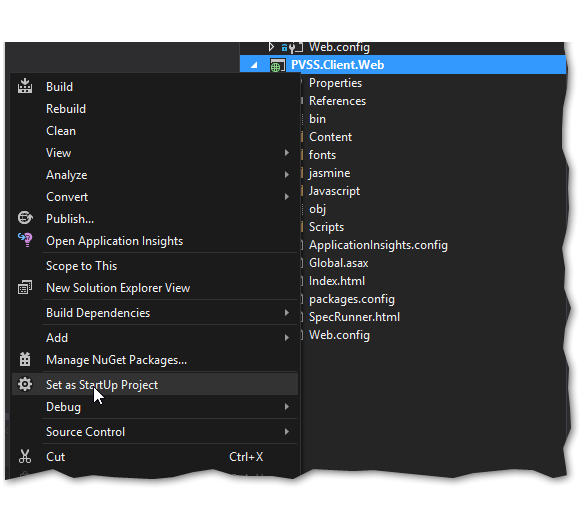
\includegraphics[scale=0.5]{Visual_Studio_small.png}}
        \caption{Visual Studio - set start project}
    \end{figure}     
    
    \item Start the application by press F10 inside Visual Studio. 
    
    \textit{This will start both the Client web server and BulletinBoard webAPI. In the bottom right corner an icon of IIS Express should be visible, by right click this icon, it should be visuable that both web service is running }
    
    \begin{figure}[H]
        \centering
        \makebox[\textwidth]{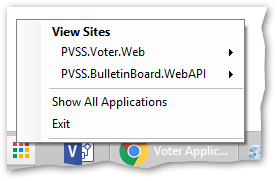
\includegraphics[scale=0.5]{IIS_Express.png}}
        \caption{Homepage}
    \end{figure}     
    
    \item When starting the application the following screen should be presented in your default browser as illustrated below. Alternatively if the programs runs in the visual studio, then paste this url http://localhost:5751/ into a browser. 
    
    \begin{figure}[H]
        \centering
        \makebox[\textwidth]{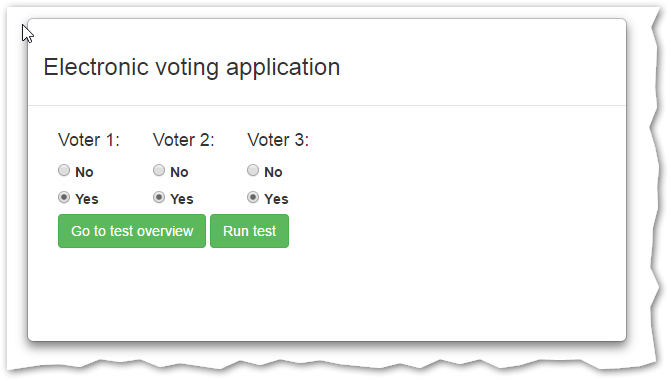
\includegraphics[scale=0.5]{Index_page.png}}
        \caption{Homepage}
    \end{figure} 
    
    
    \item By clicking the button [Run test] an election will start with 3 voters. 
    
    \textit{Hereafter a log of all the actions in the electronic voting scheme will be listed below. It is possible to change what the voters vote by clicking on the radio buttons. By default all voters votes "yes". }  
    
    \begin{figure}[H]
        \centering
        \makebox[\textwidth]{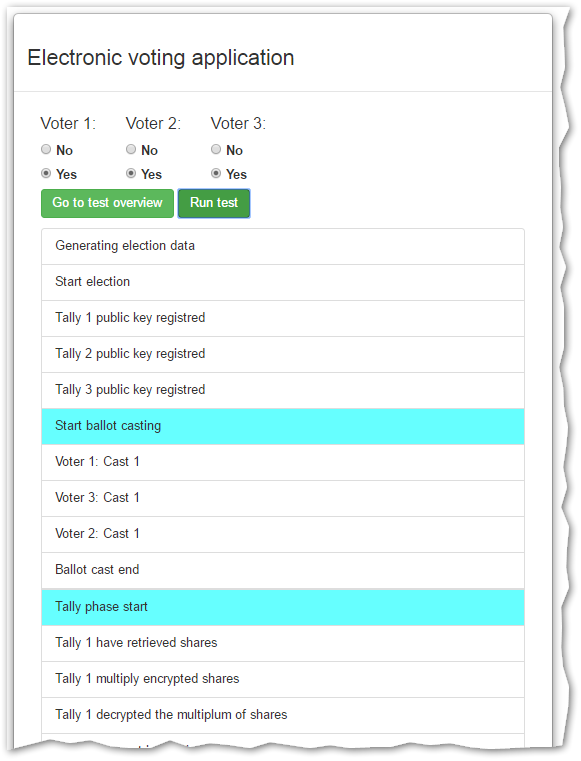
\includegraphics[scale=0.5]{Index_page_with_result.png}}
        \caption{Homepage with result}
    \end{figure} 
    
    \item Navigate to Jasmine tests by clicking the [Go to test overview] on the homepage
    
    \textit{This page shows the test results of the unit tests define in PVSS.Client\\.Web.jasmine.spec}

    \begin{figure}[H]
        \centering
        \makebox[\textwidth]{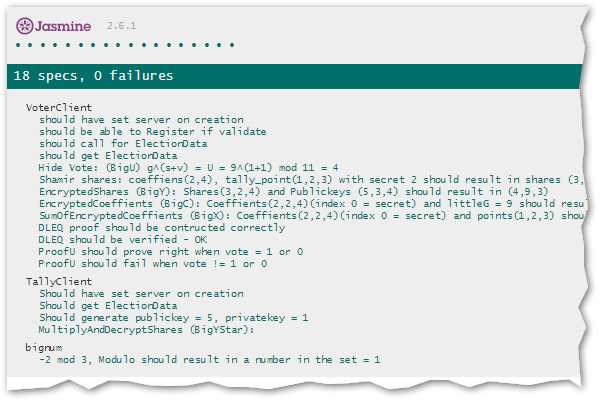
\includegraphics[scale=0.5]{SpecRunner_page.png}}
        \caption{Jasmine testpage}
    \end{figure} 
    
\end{enumerate}





 
 




